
\documentclass[UTF8]{ctexart}

\usepackage{float}
\usepackage{amsmath}
\usepackage{cases}
\usepackage{cite}
\usepackage{graphicx}
\usepackage[margin=1in]{geometry}
\geometry{a4paper}
\usepackage{fancyhdr}
\pagestyle{fancy}
\fancyhf{}


\title{{\Huge 系统基础开发工具{\large\linebreak\\}}{\Large 实验二\linebreak\linebreak}}
%please write your name, Student #, and Class # in Authors, student ID, and class # respectively
\author{\\姓\ 名:陈\ 佳\ 玲\\
学\ 号: 23100021002\\
专\ 业:23级环境工程\\
}
\date{\today}

\newpage

\begin{document}

\pagenumbering{arabic}

%\begin{document}

\fancyhead[C]{系统基础开发工具}
\fancyfoot[C]{\thepage}

\maketitle
\tableofcontents
\newpage

\section{实验目的}
 \begin{enumerate}
    \item 掌握Python程序调试的基本方法和工具,学习性能分析和优化的技术
    
    \item 理解元编程的概念和应用场景,掌握Python中代码生成和动态执行的技巧
    
    \item 掌握PyTorch框架的基本操作和核心概念,理解张量运算和自动求导机制,学会构建和训练神经网络模型
\end{enumerate}


\section{实验内容}

\subsection{调试与性能分析}

\subsubsection{获取超级用户登录信息及所执行的指令}
使用 Linux 上的 journalctl 命令来获取最近一天中超级用户的登录信息及其所执行的指令
\begin{figure}[H]
    \centering
    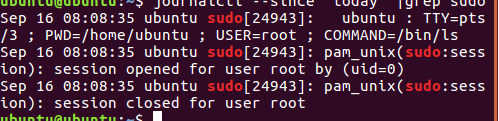
\includegraphics[width=0.95\textwidth]{picture/查看日志.png}
    \caption{获取超级用户登录信息}
\end{figure}

\subsubsection{打印调试法与日志}
创建一个日志文件logger.py执行不同的指令使得输出不同的结果信息。
\begin{figure}[H]
    \centering
    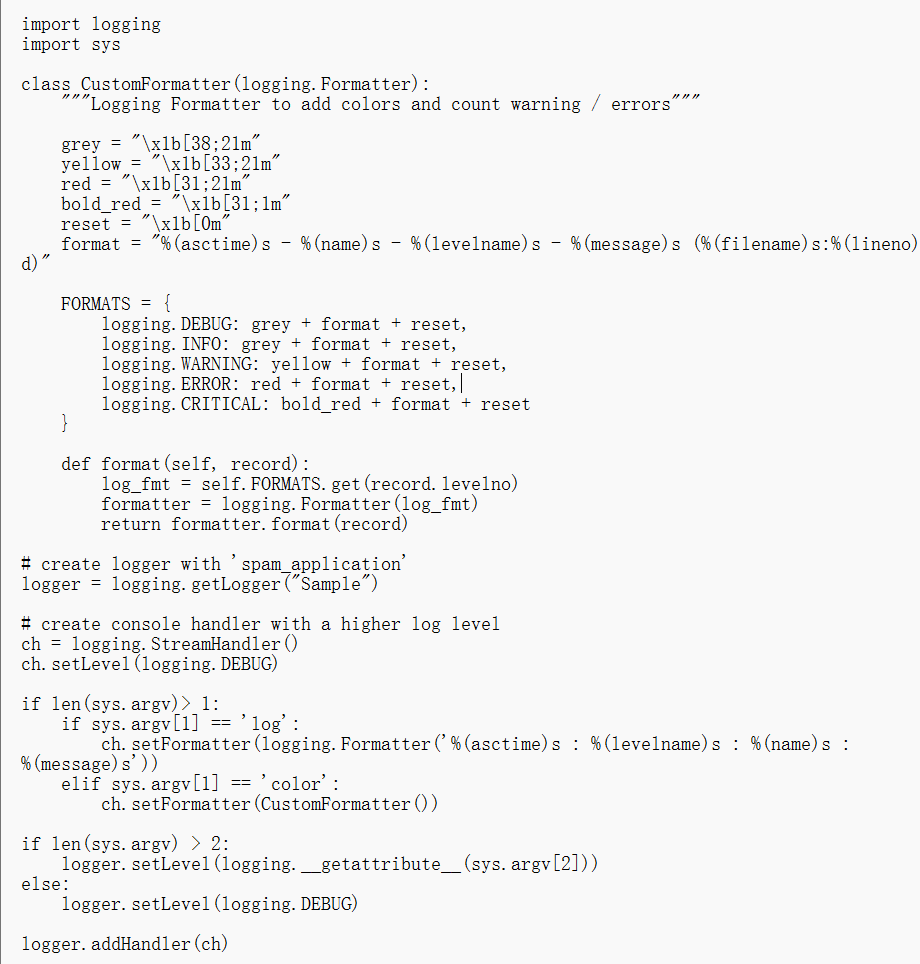
\includegraphics[width=0.95\textwidth]{picture/日志文件.png}
    \caption{logger.py}
\end{figure}
\begin{enumerate}
    \item 直接使用 print() 语句输出的内容,没有经过任何日志格式化或级别过滤。
    \begin{figure}[H]
    \centering
    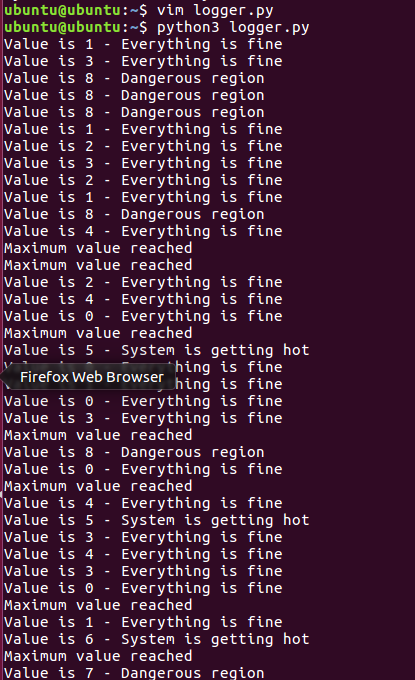
\includegraphics[width=0.95\textwidth]{picture/直接打印.png}
    \caption{无格式化}
\end{figure}
    \item 仅经过日志格式化(Log formatted output)的输出。通常会包含时间戳、日志级别(如INFO、ERROR)、模块名等信息,结构更清晰,易于后续分析。
    \begin{figure}[H]
    \centering
    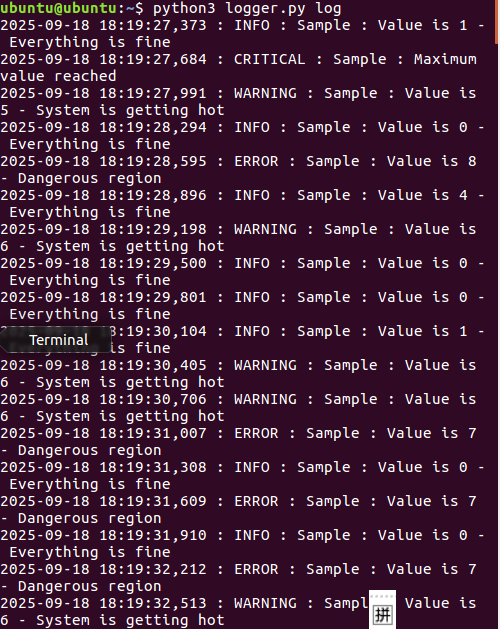
\includegraphics[width=0.95\textwidth]{picture/2.png}
    \caption{日志格式化}
\end{figure}
    
    
    \item 仅输出日志级别为 ERROR 及以上(如ERROR、CRITICAL)的信息。过滤掉较低级别的日志(如DEBUG、INFO、WARNING),只显示错误和严重错误信息,便于快速定位问题
    \begin{figure}[H]
    \centering
    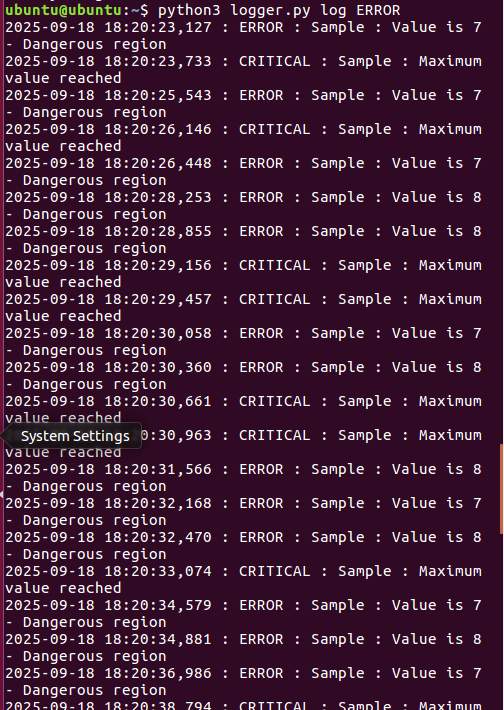
\includegraphics[width=0.95\textwidth]{picture/3.png}
    \caption{输出日志级别ERROR以上的}
\end{figure}
    
    \item :彩色格式化输出(Color formatted output).不同级别的日志会以不同颜色显示(如ERROR用红色,WARNING用黄色),增强可读性,适合在终端中实时查看
    \begin{figure}[H]
    \centering
    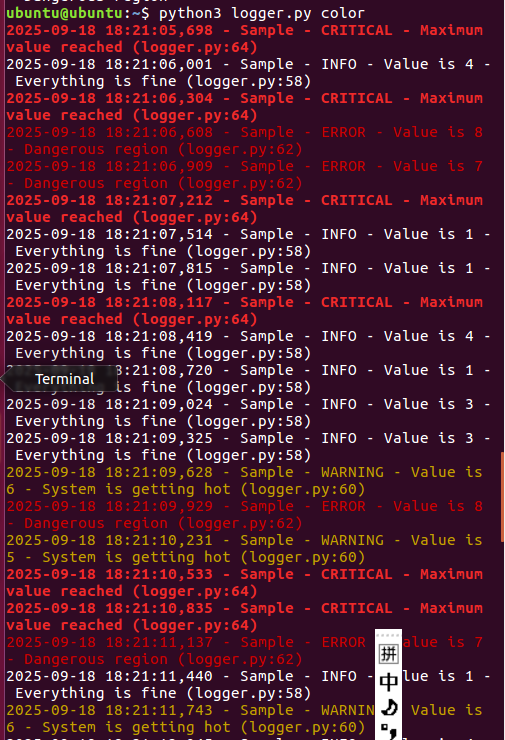
\includegraphics[width=0.95\textwidth]{picture/4.png}
    \caption{彩色格式化输出}
\end{figure}

\end{enumerate}





\subsubsection{ python调试器——pdb}
pdb 是 Python 自带的一个强大的交互式源代码调试器。它允许你在程序任意位置设置断点、单步执行、查看变量值、查看调用栈,甚至动态修改变量和执行代码,是排查复杂 Bug 的终极利器。
\begin{figure}[H]
    \centering
    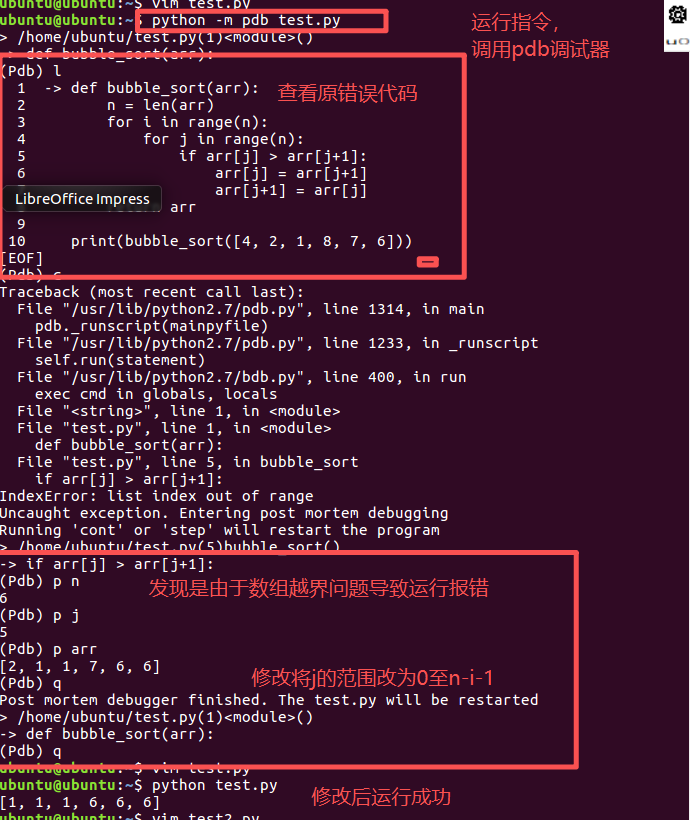
\includegraphics[width=0.95\textwidth]{picture/调试器操作流程.png}
    \caption{调试器pdb的操作}
\end{figure}

\subsubsection{性能分析——计时}
 Python 的 time 模块:
 (1)真实时间 Real - 从程序开始到结束流失掉的真实时间,包括其他进程的执行时间以及阻塞消耗的时间(例如等待 I/O 或网络)//
(2)用户时间 User - CPU 执行用户代码所花费的时间//
(3)系统时间 Sys - CPU 执行系统内核代码所花费的时间。
\begin{figure}[H]
    \centering
    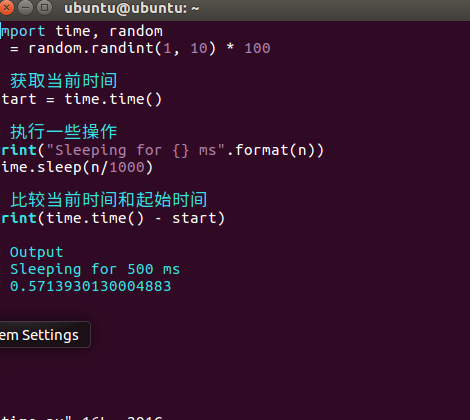
\includegraphics[width=0.95\textwidth]{picture/时间分析代码.png}
    \caption{时间分析代码}
\end{figure}

\begin{figure}[H]
    \centering
    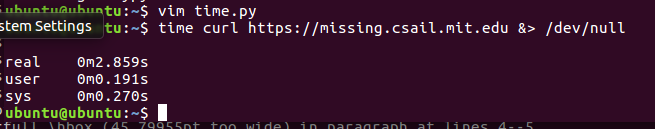
\includegraphics[width=0.95\textwidth]{picture/时间分析操作运行.png}
    \caption{时间分析操作}
\end{figure}



\subsection{元编程}
\subsubsection{构建系统}
make 是最常用的构建系统之一,它通常被安装到了几乎所有基于 UNIX 的系统中。当执行 make 时,它会去参考当前目录下名为 Makefile 的文件。
\begin{figure}[H]
    \centering
    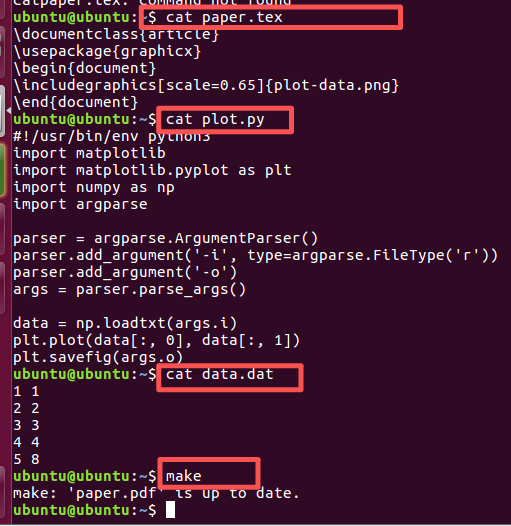
\includegraphics[width=0.95\textwidth]{picture/make.png}%保证图片占满页面宽度,且一致
    \caption{make构建系统简单操作}
\end{figure}

\subsubsection{类装饰器}

\begin{figure}[H]
    \centering
    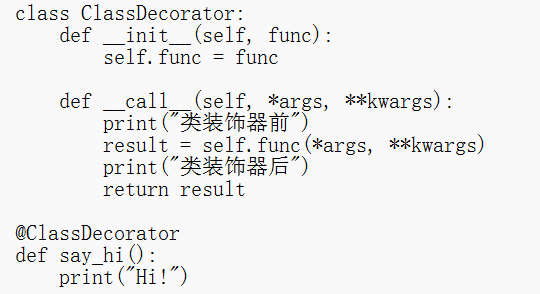
\includegraphics[width=0.95\textwidth]{picture/类装饰器的创建.png}%保证图片占满页面宽度,且一致
    \caption{类装饰器}
\end{figure}

\subsection{Pytorch}

\subsubsection{PyTorch 张量} 
张量是一个多维数组,可以是标量、向量、矩阵或更高维度的数据结构。在 PyTorch 中,张量是数据的核心表示形式,类似于 NumPy 的多维数组,但具有更强大的功能,例如支持 GPU 加速和自动梯度计算。张量支持多种数据类型(整型、浮点型、布尔型等)。张量可以存储在 CPU 或 GPU 中,GPU 张量可显著加速计算。

\begin{figure}[H]
    \centering
    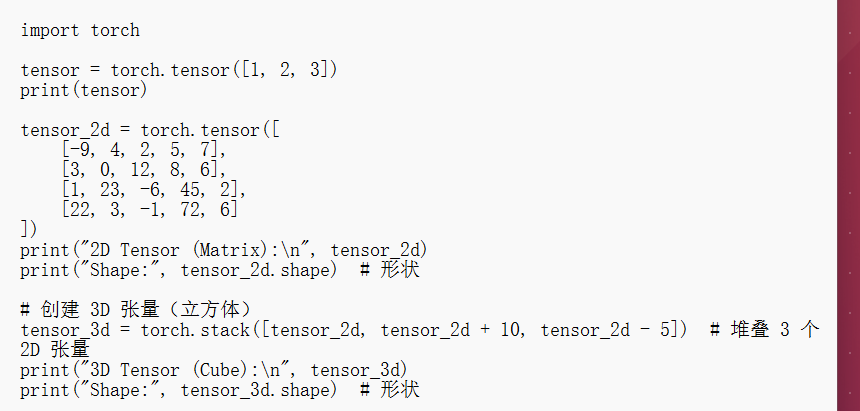
\includegraphics[width=0.95\textwidth]{picture/创建张量代码.png}%保证图片占满页面宽度,且一致
    \caption{张量的声明与定义}
\end{figure}

\begin{figure}[H]
    \centering
    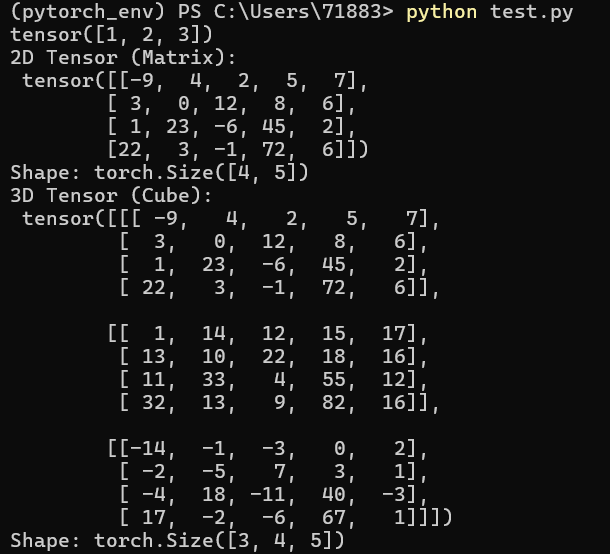
\includegraphics[width=0.95\textwidth]{picture/创建张量执行结果.png}%保证图片占满页面宽度,且一致
    \caption{张量的创建结果}
\end{figure}

\subsubsection{张量形状操作}

\begin{figure}[H]
    \centering
    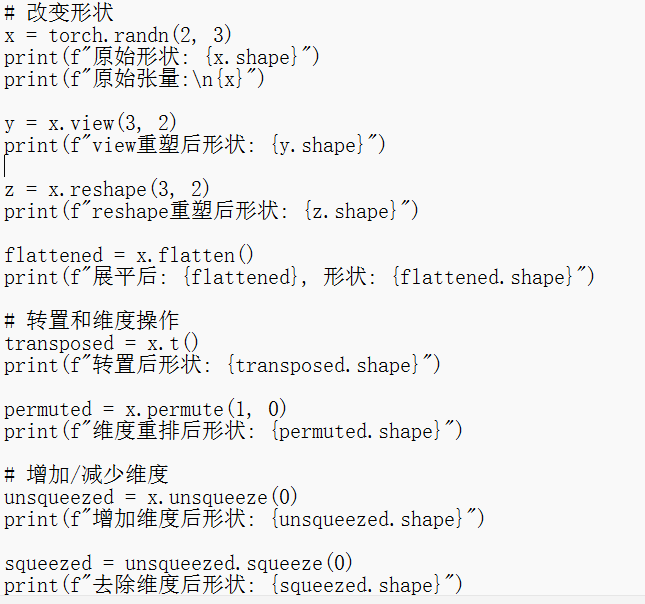
\includegraphics[width=0.95\textwidth]{picture/改变张量形状.png}%保证图片占满页面宽度,且一致
    \caption{改变张量形状}
\end{figure}


\begin{figure}[H]
    \centering
    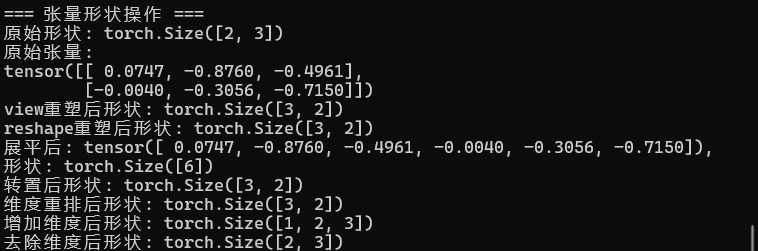
\includegraphics[width=0.95\textwidth]{picture/张量形状改变结果.png}%保证图片占满页面宽度,且一致
    \caption{改变后结果}
\end{figure}
\subsubsection{张量运算的三种实现方法}
1. 三种运算方式的区别\\
(1)运算符方式:a + b - 最直观,创建新张量\\
(2)函数方式:torch.add(a, b) - 功能更丰富,可指定输出张量\\
(3)原地操作:a.add_(b) - 修改原张量,节省内存
\begin{figure}[H]
    \centering
    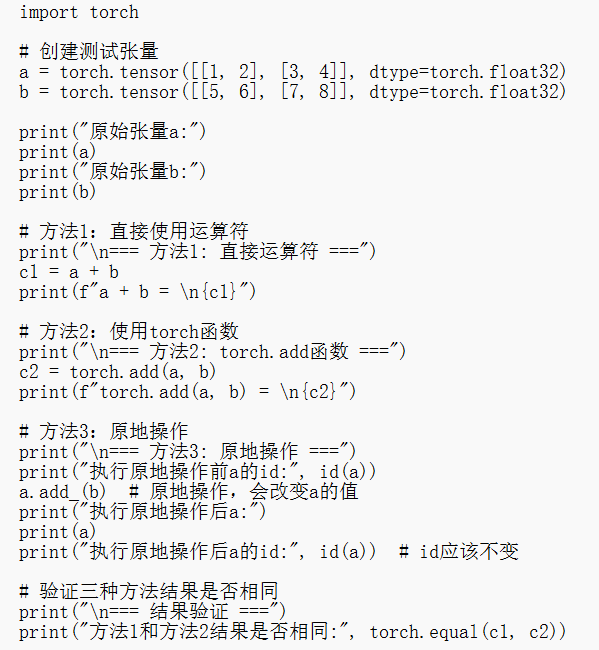
\includegraphics[width=0.95\textwidth]{picture/三种运算方法代码.png}%保证图片占满页面宽度,且一致
    \caption{三种运算方法示例}
\end{figure}

\begin{figure}[H]
    \centering
    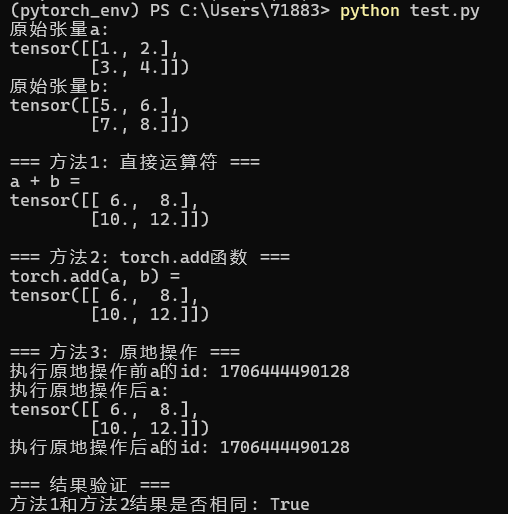
\includegraphics[width=0.95\textwidth]{picture/三种运算结果.png}%保证图片占满页面宽度,且一致
    \caption{运算结果}
\end{figure}

\subsubsection{自动求导}
\begin{figure}[H]
    \centering
    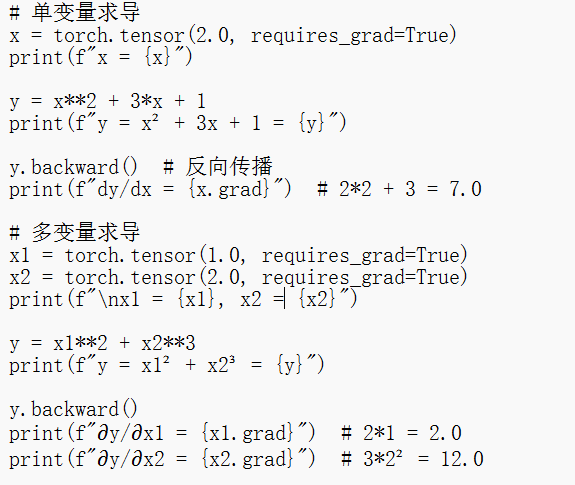
\includegraphics[width=0.95\textwidth]{picture/自动求导示例.png}%保证图片占满页面宽度,且一致
    \caption{自动求导方法}
\end{figure}
\begin{figure}[H]
    \centering
    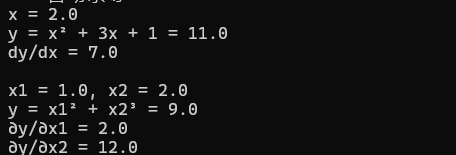
\includegraphics[width=0.95\textwidth]{picture/自动求导.png}%保证图片占满页面宽度,且一致
    \caption{运行效果图}
\end{figure}


\subsubsection{Tensor与Numpy数组的相互转换}
PyTorch张量和NumPy数组可以共享底层内存,必要条件是张量必须在CPU上,且数据类型兼容,能够避免数据拷贝,提高效率
\begin{figure}[H]
    \centering
    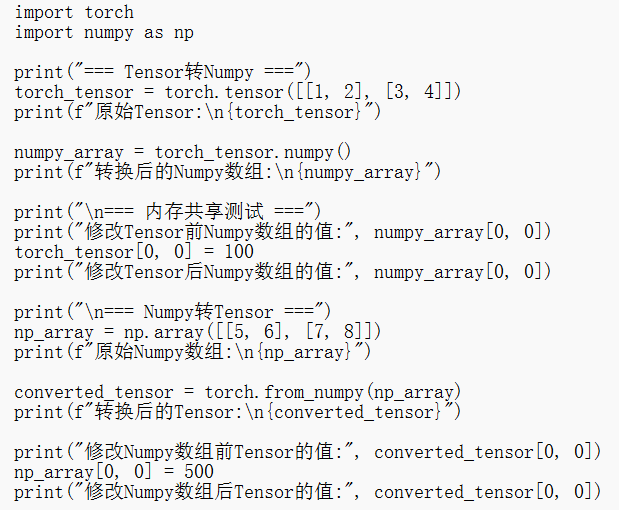
\includegraphics[width=0.95\textwidth]{picture/Tensor与Numpy数组的相互转换.png}%保证图片占满页面宽度,且一致
    \caption{转换代码示例}
\end{figure}
 \begin{figure}[H]
    \centering
    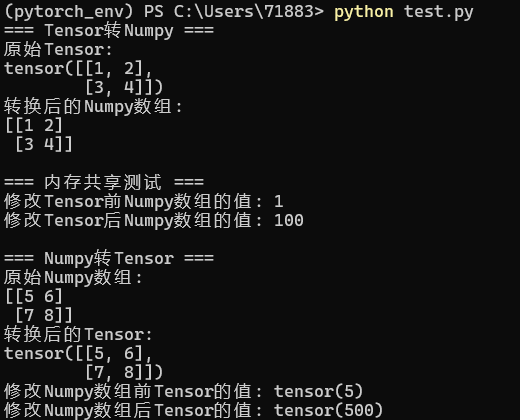
\includegraphics[width=0.95\textwidth]{picture/Tensor与Numpy数组的相互转换前后比对结果.png}%保证图片占满页面宽度,且一致
    \caption{转换前后结果对比}
\end{figure}

\subsubsection{自动梯度计算}
使用直接调用backward(),需要传入梯度参数后计算
\begin{figure}[H]
    \centering
    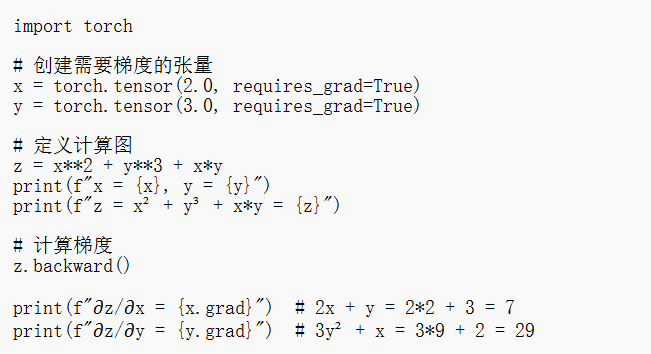
\includegraphics[width=0.95\textwidth]{picture/梯度计算代码.png}%保证图片占满页面宽度,且一致
    \caption{梯度计算方法}
\end{figure}

\begin{figure}[H]
    \centering
    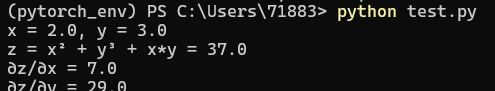
\includegraphics[width=0.95\textwidth]{picture/梯度计算结果.png}%保证图片占满页面宽度,且一致
    \caption{计算梯度结果}
\end{figure}

\subsubsection{自定义简单神经网络}
nn.Module是所有神经网络模块的基类,封装了参数管理、设备转移等功能。前向传播定义数据流动路径,支持复杂逻辑
(1)nn.Module基类,采用模块化设计,是所有神经网络模块的基类,自动跟踪所有可训练参数并处理CPU/GPU设备转移,支持模型保存和加载。\\
(2)采用前向传播设计,forward方法定义数据流动路径。支持条件判断、循环等复杂逻辑\\
\begin{figure}[H]
    \centering
    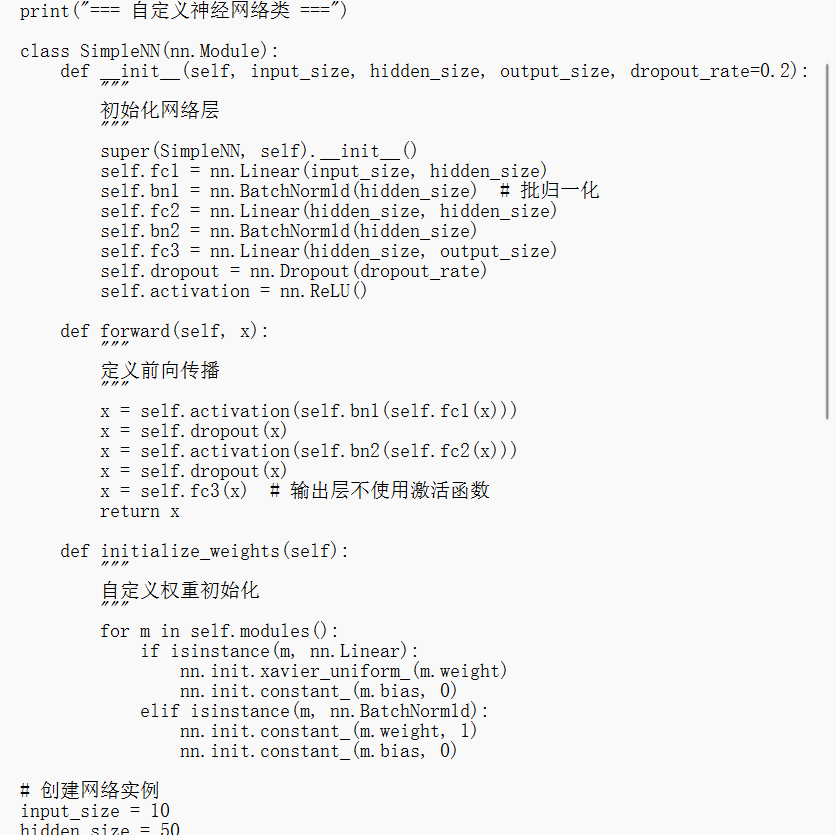
\includegraphics[width=0.95\textwidth]{picture/自定义神经网络代码.png}%保证图片占满页面宽度,且一致
    \caption{自定义神经网络的主体代码}
\end{figure}

\begin{figure}[H]
    \centering
    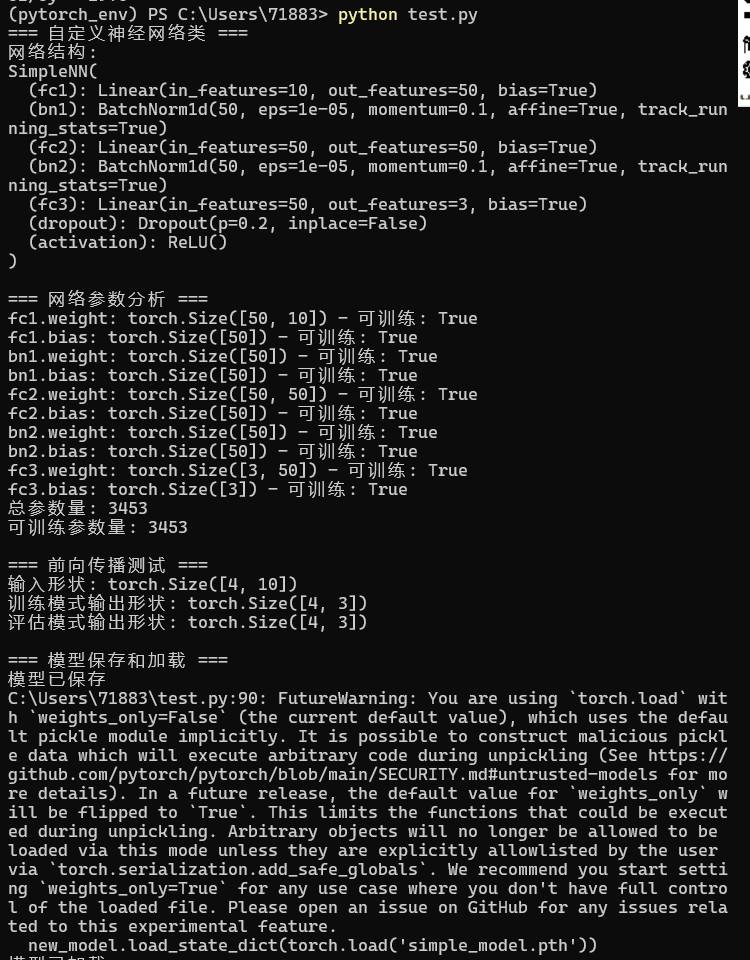
\includegraphics[width=0.95\textwidth]{picture/自定义神经网络.png}%保证图片占满页面宽度,且一致
    \caption{自定义神经网络}
\end{figure}

\subsubsection{常用损失函数的使用}
损失函数衡量模型预测与真实值的差异,MSE适用于回归任务,交叉熵适用于分类任务。理解不同损失函数的数学特性和适用场景对模型训练至关重要,合适的损失函数能有效引导模型学习方向
\begin{figure}[H]
    \centering
    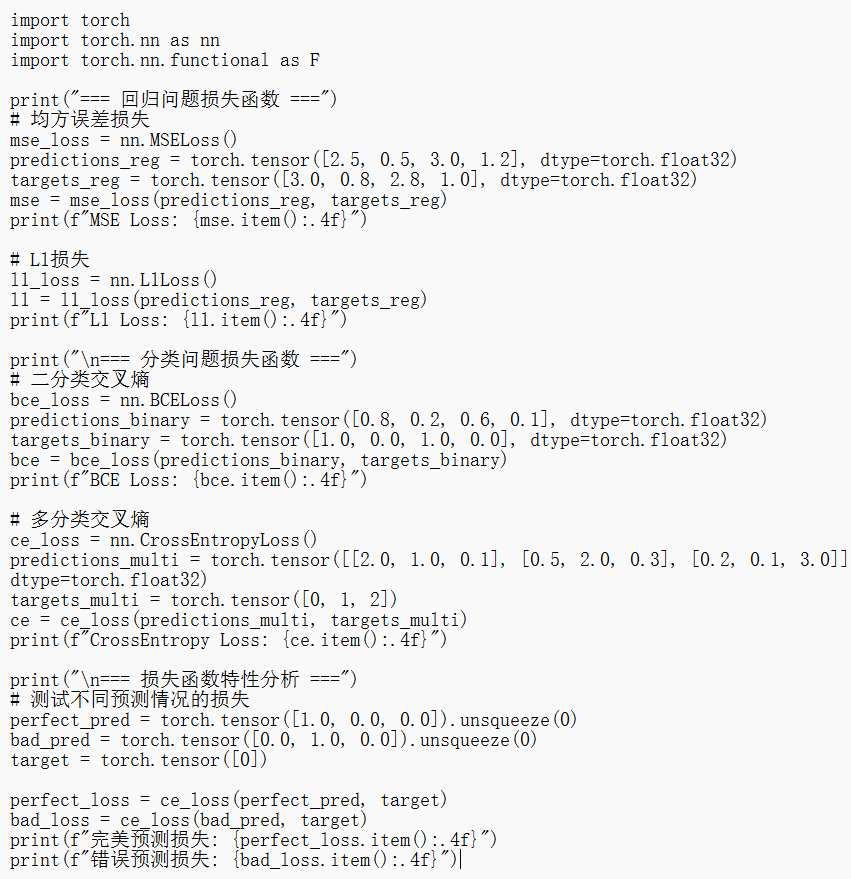
\includegraphics[width=0.95\textwidth]{picture/损失函数的使用.png}%保证图片占满页面宽度,且一致
    \caption{损失函数使用方法}
\end{figure}

\begin{figure}[H]
    \centering
    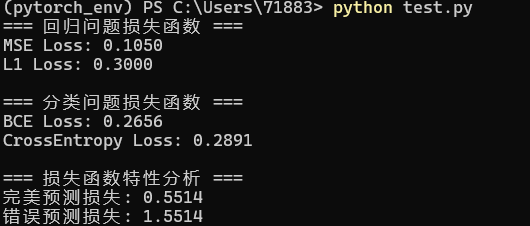
\includegraphics[width=0.95\textwidth]{picture/损失函数使用结果.png}%保证图片占满页面宽度,且一致
    \caption{损失函数使用结果}
\end{figure}

\subsubsection{反向传播流程实践}
反向传播是基于链式法则的梯度计算方法,通过计算图从输出向输入逐层传播误差。梯度清零防止累加,数值梯度验证确保实现正确性。
\begin{figure}[H]
    \centering
    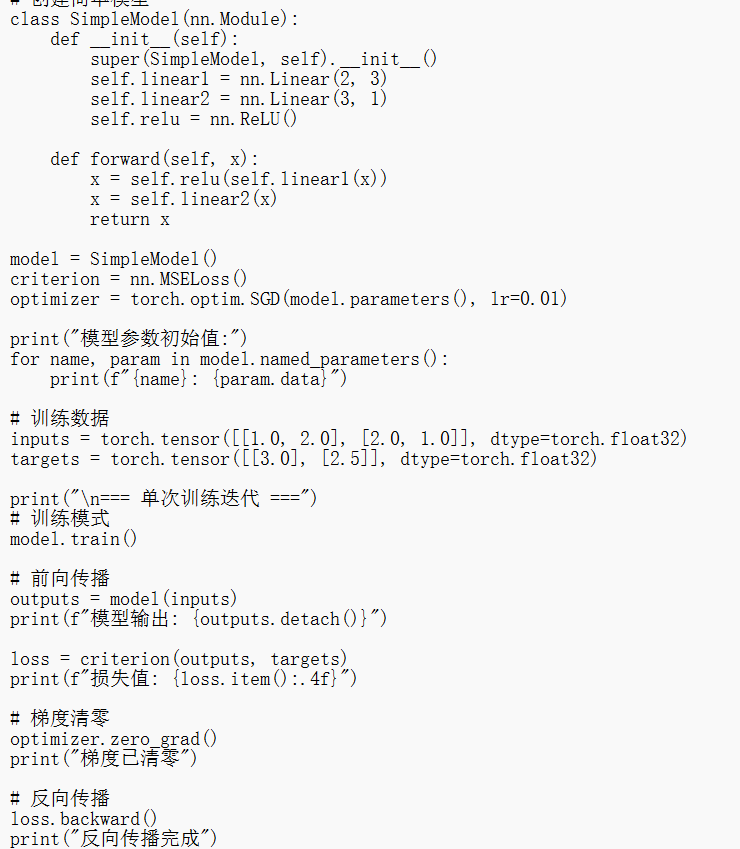
\includegraphics[width=0.95\textwidth]{picture/反向传播简单实现.png}%保证图片占满页面宽度,且一致
    \caption{反向传播简单实现}
\end{figure}

\begin{figure}[H]
    \centering
    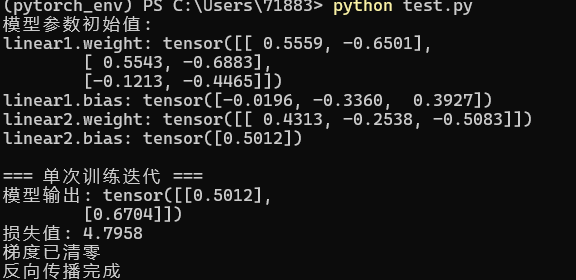
\includegraphics[width=0.95\textwidth]{picture/反向传播结果.png}%保证图片占满页面宽度,且一致
    \caption{反向传播结果}
\end{figure}

\subsubsection{优化器与权重更新}
优化器根据梯度更新模型参数,SGD简单但可能收敛慢,带动量的SGD加速收敛,Adam自适应调整学习率。学习率调度动态调整学习率,权重衰减防止过拟合

\begin{figure}[H]
    \centering
    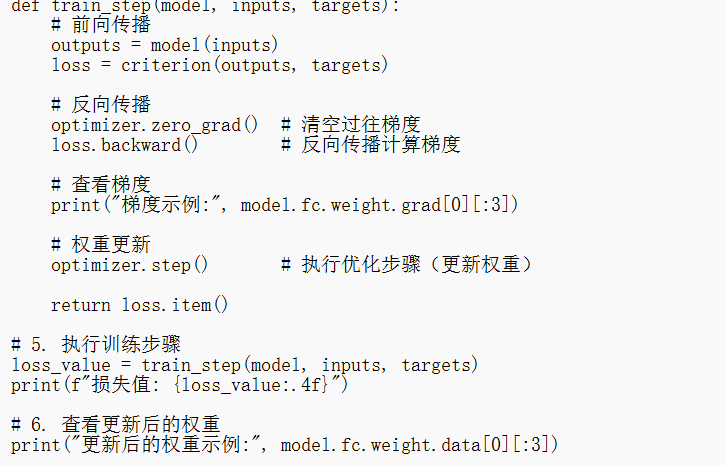
\includegraphics[width=0.95\textwidth]{picture/优化器简单使用.png}%保证图片占满页面宽度,且一致
    \caption{优化器简单使用}
\end{figure}
\begin{figure}[H]
    \centering
    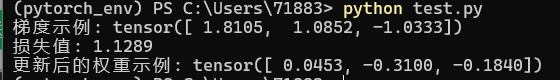
\includegraphics[width=0.95\textwidth]{picture/权重更新的简单使用.png}%保证图片占满页面宽度,且一致
    \caption{权重更新结果}
\end{figure}

\subsubsection{CIFAR10数据加载和预处理}
下载CIFAR10数据集,定义数据变换,创建DataLoader,实现批量数据加载。
数据加载是模型训练的前提,DataLoader提供批量加载、打乱、并行加载等功能。数据预处理包括归一化、数据增强等,对模型性能有重要影响
\begin{figure}[H]
    \centering
    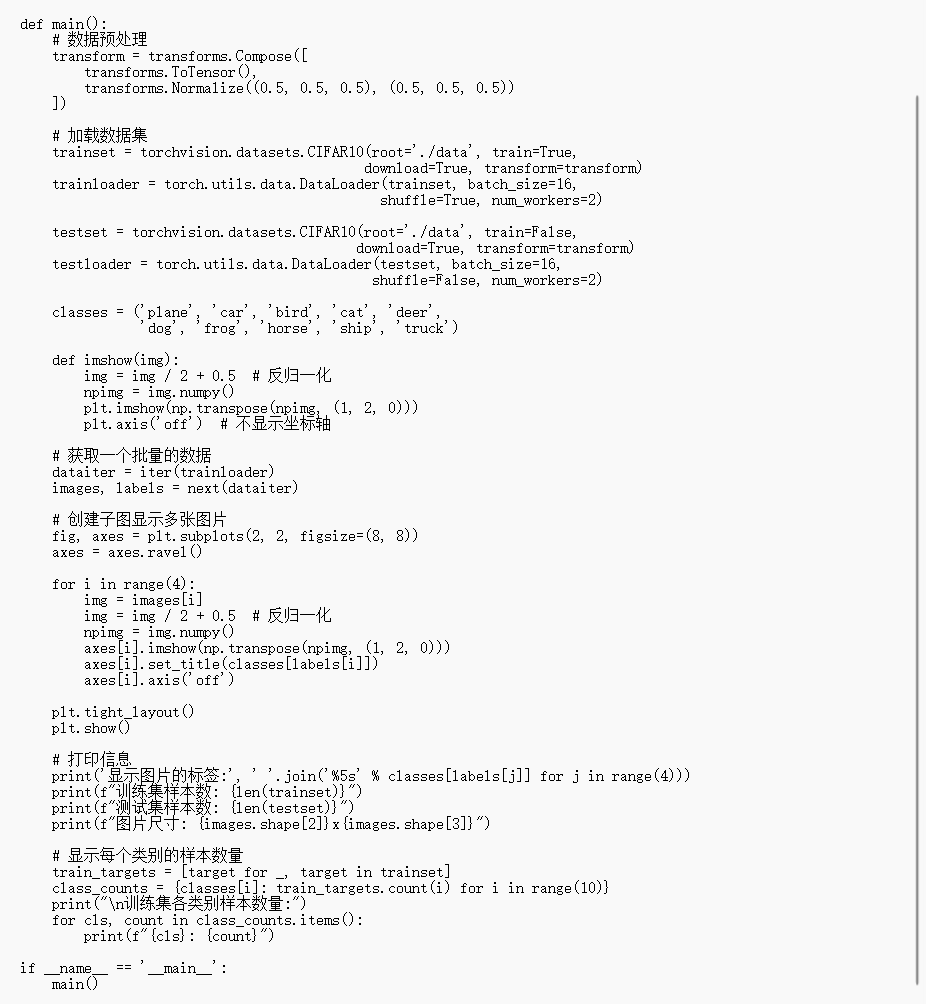
\includegraphics[width=0.95\textwidth]{picture/CIFAR10数据加载和预处理.png}%保证图片占满页面宽度,且一致
    \caption{处理代码}
\end{figure}

(2)删除和修改元组
\begin{figure}[H]
    \centering
    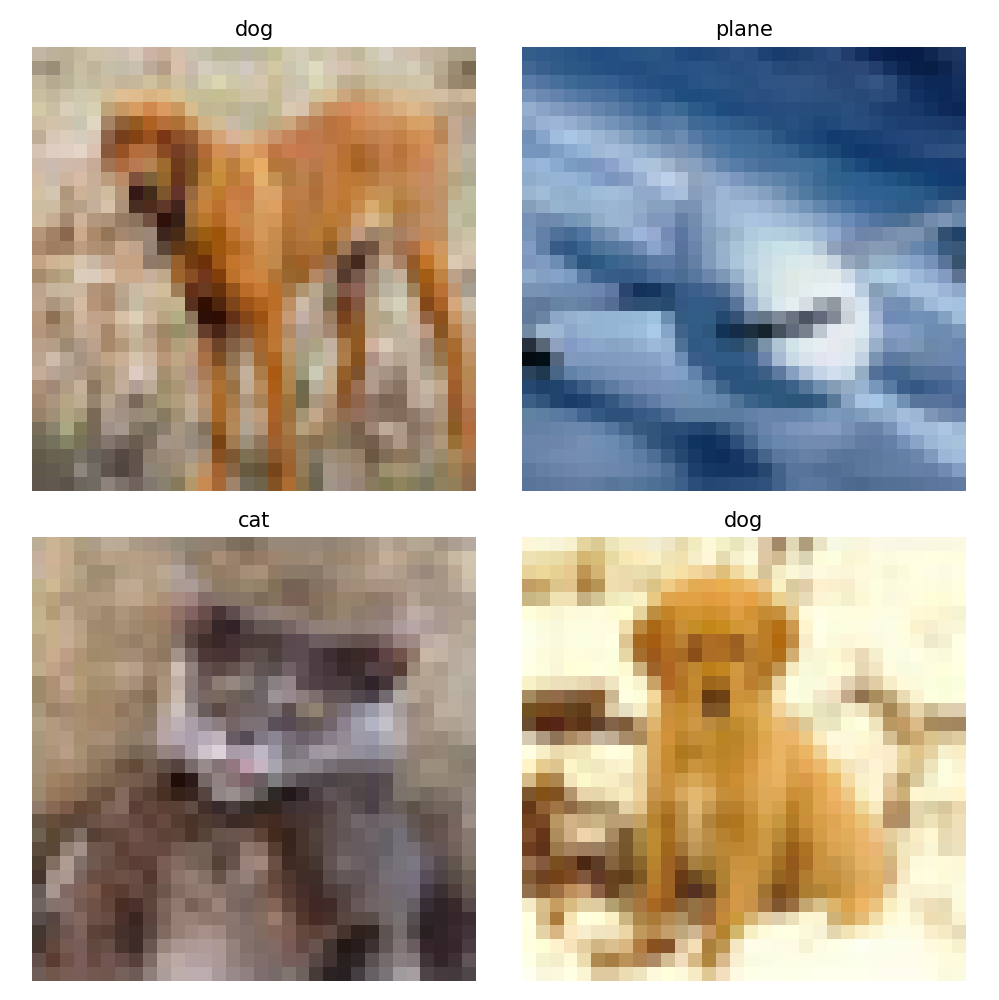
\includegraphics[width=0.95\textwidth]{picture/处理结果.png}%保证图片占满页面宽度,且一致
    \caption{处理结果}
\end{figure}


\subsubsection{卷积操作}

\begin{figure}[H]
    \centering
    
\includegraphics[width=0.95\textwidth]{picture/卷积操作.png}%保证图片占满页面宽度,且一致
    \caption{卷积操作}
\end{figure}
\begin{figure}[H]
    \centering
    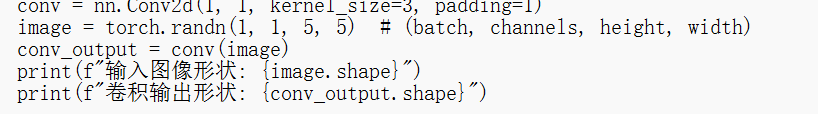
\includegraphics[width=0.95\textwidth]{picture/卷积操作代码.png}%保证图片占满页面宽度,且一致
    \caption{卷积操作效果图}
\end{figure}


\subsubsection{卷积神经网络简单实现}
\begin{figure}[H]
    \centering
    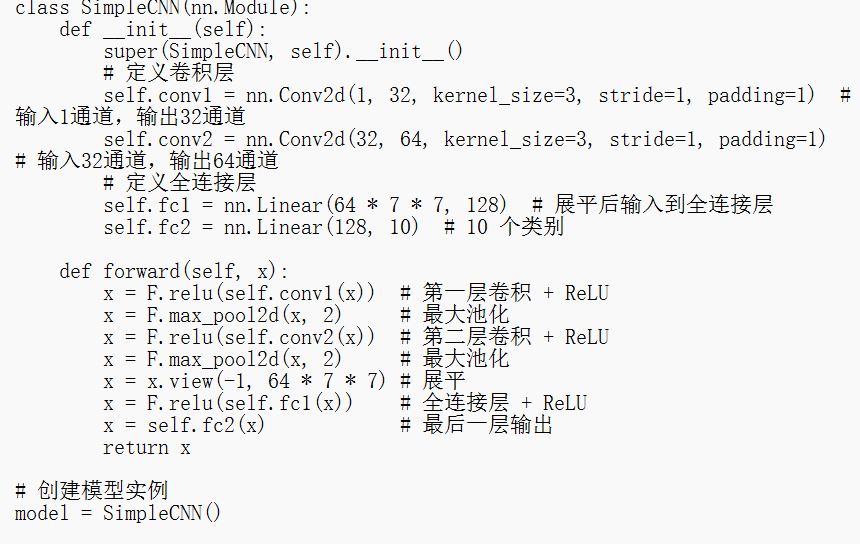
\includegraphics[width=0.95\textwidth]{picture/卷积神经网络.png}%保证图片占满页面宽度,且一致
    \caption{简单实现}
\end{figure}




\subsubsection{测试代码以及可视化结果}
\begin{figure}[H]
    \centering
    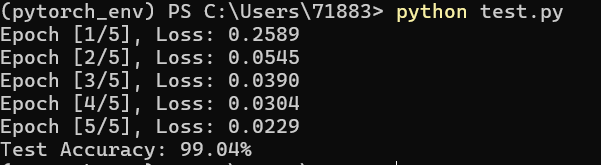
\includegraphics[width=0.95\textwidth]{picture/训练数据准确率.png}%保证图片占满页面宽度,且一致
    \caption{训练数据}
\end{figure}
\begin{figure}[H]
    \centering
    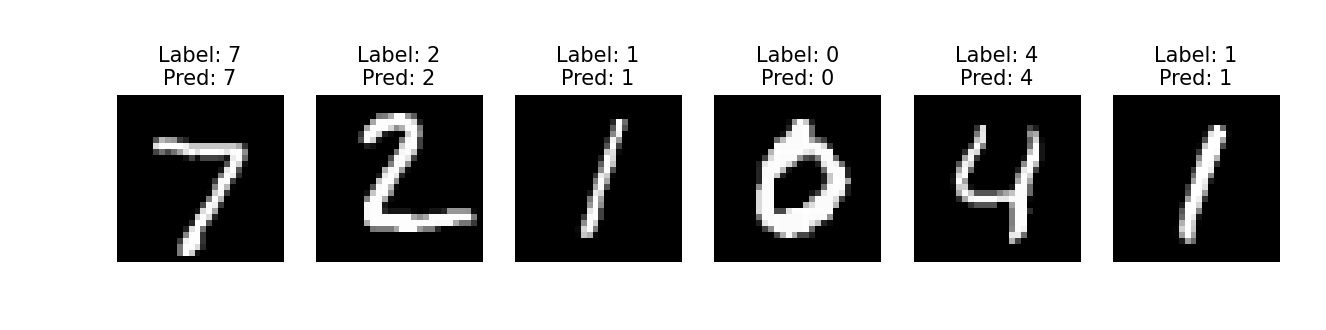
\includegraphics[width=0.95\textwidth]{picture/可视化结构.png}%保证图片占满页面宽度,且一致
    \caption{可视化结果}
\end{figure}
\section{心得体会}
在本次的实验当中,从调试与性能分析当中学习基础调试工具,动手实践学习,感受如何系统化地定位和解决问题;在元编程的实践中,知道什么是元编程以及代码抽象;在Pytorch的部分,学习相关的基础语法知识,拓宽了视野,有助于以后的学习。


\section{实验代码查看链接}
本次报告相关练习、报告和代码均可以在https://github.com/chen2-spec/my-latex-report查看



\end{document}
